% Copyright (c) 2026 Islam Ibrahim. All rights reserved.

\documentclass[tikz,border=10pt]{standalone}
\usepackage[T1]{fontenc}
\usepackage{lmodern}
\usepackage{amsmath}
\usepackage{tikz}
\usetikzlibrary{arrows.meta,positioning,calc}

\begin{document}
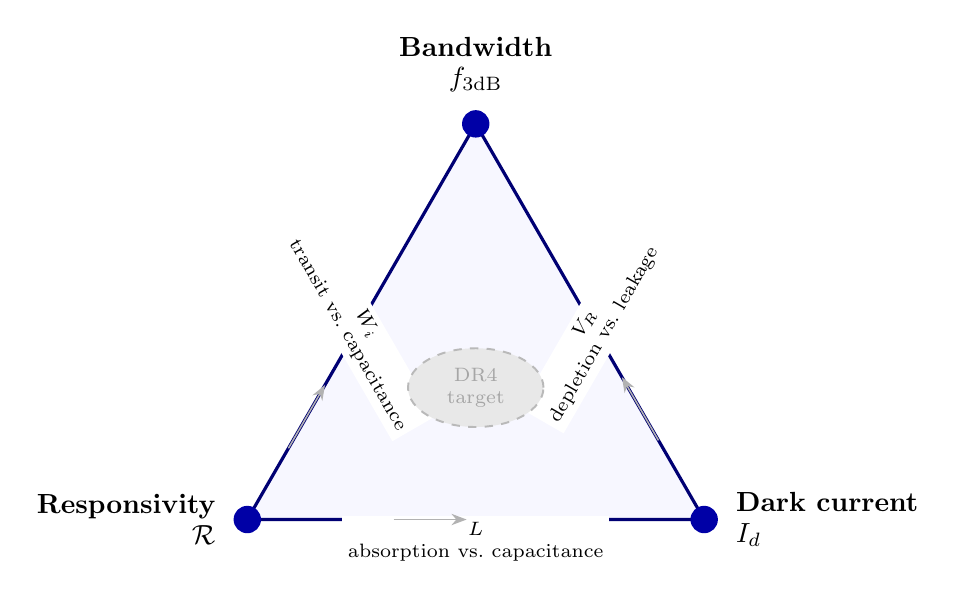
\begin{tikzpicture}[font=\small\rmfamily,>=Stealth,
  lbl/.style={font=\scriptsize\rmfamily,align=center},
  vtx/.style={circle,fill=blue!65!black,inner sep=3.5pt},
  lever/.style={font=\scriptsize\rmfamily,align=center,fill=white,inner sep=2pt},
]

\def\R{3.35}
\coordinate (BW) at (90:\R);
\coordinate (RESP) at (210:\R);
\coordinate (NOISE) at (330:\R);
\coordinate (C) at (0,0);

\fill[blue!3] (BW)--(RESP)--(NOISE)--cycle;
\draw[line width=1.15pt,blue!45!black] (BW)--(RESP)--(NOISE)--cycle;
\node[vtx] at (BW) {};
\node[vtx] at (RESP) {};
\node[vtx] at (NOISE) {};

\node[font=\normalsize\bfseries\rmfamily,align=center,above=8pt] at (BW)
  {Bandwidth\\[-1pt]$f_{3\mathrm{dB}}$};
\node[font=\normalsize\bfseries\rmfamily,align=right,left=8pt] at (RESP)
  {Responsivity\\[-1pt]$\mathcal{R}$};
\node[font=\normalsize\bfseries\rmfamily,align=left,right=8pt] at (NOISE)
  {Dark current\\[-1pt]$I_d$};

% Keep the edge text compact; detailed physics belongs in the caption.
\node[lever,rotate=-60] at ($(BW)!0.52!(RESP)$) {$W_i$\\transit vs.\ capacitance};
\node[lever,rotate=60] at ($(BW)!0.52!(NOISE)$) {$V_R$\\depletion vs.\ leakage};
\node[lever] at ($(RESP)!0.50!(NOISE)+(0,-0.28)$) {$L$\\absorption vs.\ capacitance};

\fill[gray!18,draw=gray!55,dashed,line width=0.7pt] (C) ellipse (0.86cm and 0.50cm);
\node[lbl,gray!70] at (C) {DR4\\target};

\draw[->,line width=0.55pt,gray!60] ($(RESP)!0.18!(BW)$) -- ($(RESP)!0.34!(BW)$);
\draw[->,line width=0.55pt,gray!60] ($(NOISE)!0.20!(BW)$) -- ($(NOISE)!0.36!(BW)$);
\draw[->,line width=0.55pt,gray!60] ($(RESP)!0.32!(NOISE)$) -- ($(RESP)!0.48!(NOISE)$);

\end{tikzpicture}
\end{document}
